\section{Introduction}
\frame{\sectionpage}

\begin{frame}{Inspiration}
    \uncover<+->{Immigration court ruling}
    \uncover<+->{
        \begin{itemize}
            \item<+-> High stake: granted asylum or deported
            \item<+-> Simple structure: lower court and appeal court
            \item<+-> Idiosyncratic decisions: one single judge makes the decision
        \end{itemize}
    }
    
    \uncover<+->{
        \vspace*{15pt}
        Are judges doing their job \textbf{\color{goldenrod}careful} enough?
    }
    
\end{frame}

\begin{frame}{This study}

    I focus on the \textcolor<2->{goldenrod}{\textbf{inattention}} of lower court judges, and 
    
    \begin{columns}[T]

        \begin{column}{0.45\textwidth}
            \uncover<2->{\begin{block}{\small \centering \textbf{Prediction}}
            \uncover<3->{
                \begin{itemize}
                    \item Lower court decisions: are judges predictable?
                    \item Appeal results: how they react to reverse
                \end{itemize}
            
            }
            \end{block}}
        \end{column}
        
        \begin{column}{0.45\textwidth}
            \uncover<2->{\begin{block}{\small \centering \textbf{Impact}}
            \uncover<5->{
            \begin{itemize}
                \item[-] The heterogeneity in judicial inattention
                \item[-] Can we nudge judges to pay more atention?
            \end{itemize}
            }
            \end{block}}
        \end{column}
        
        \end{columns}
\end{frame}


\begin{frame}{{A Preview}}

    \begin{itemize}
        \item<+-> \textcolor{goldenrod}{\textbf{Judges are not that attentive}}: lower-court decisions can be predicted after a particular judge is assigned, but prior to judicial inquiry into the case
        \item<+-> \textcolor{goldenrod}{\textbf{There is evdience of behavioral anomalies}}: judges show different level of early predictability
        \item<+-> \textcolor{goldenrod}{\textbf{Attentiveness can be proxied}}: leveraging appeal court decisions, I create a proxy for attentiveness of lower court judges
        \item<+-> \textcolor{goldenrod}{\textbf{Judicial inattention can be improved}}: observational evidence suggests several channels for further nudging RCTs 
    \end{itemize}
        
\end{frame}

\begin{frame}{Data}
    
\begin{columns}

\begin{column}{0.65\textwidth}
    \begin{figure}\label{fig:data_structure}
    \centering
    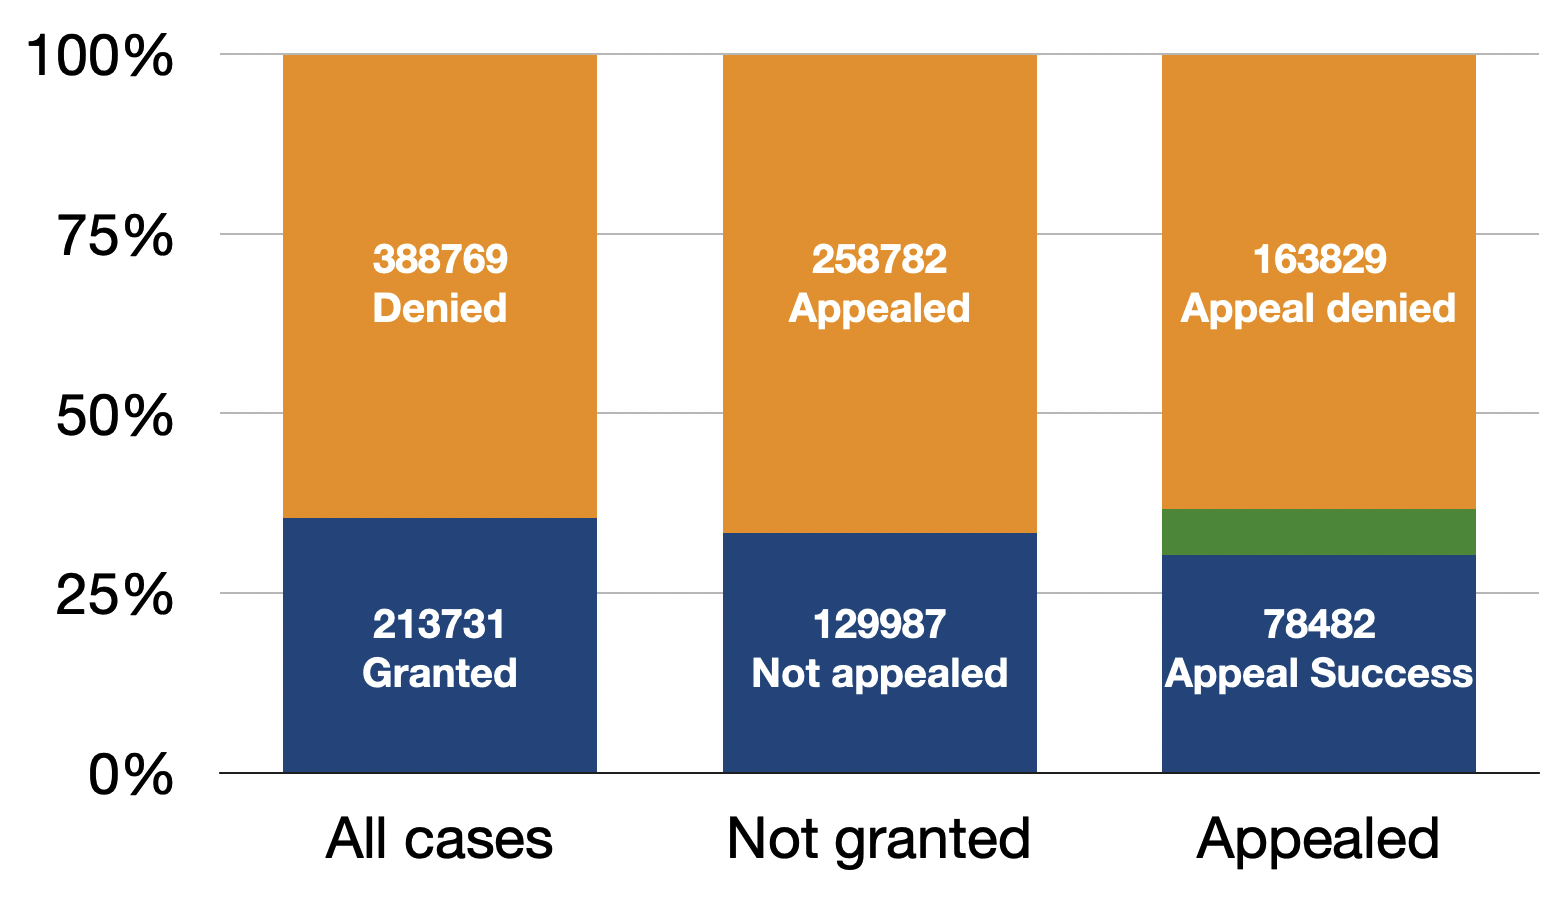
\includegraphics[height = 0.65 \textheight]{images/fig_data.png}
    \caption{Data Structure}
    \end{figure}
\end{column}

\begin{column}{0.3\textwidth}

\only<1>{
    \small
    \begin{itemize}
        \item \textbf{\color{goldenrod}Total cases}: 602500 cases (35\% granted)
        \item \textbf{\color{goldenrod}Appeal cases}: 242466 appeals (32.4\% successful) after removing recent appeals and appeal by the government
    \end{itemize}
    From \citet*{chen2016decision} and \citet*{dunn2017early}
    }

\end{column}
\end{columns}

\end{frame}

    